\documentclass[11pt,letterpaper]{article}
\usepackage[utf8x]{inputenc}
%\usepackage[spanish]{babel}
\usepackage{ucs}
\usepackage{amsmath}
\usepackage{amsfonts}
\usepackage{amssymb}
\usepackage{natbib}
%\usepackage{hyperref}
\usepackage[bookmarks]{hyperref}%,colorlinks,citecolor=black,linkcolor=black,urlcolor=black
\usepackage{appendix}
\usepackage{multirow}
%Adds ability to change enumerators:
% [I] for capital roman numbers
% [(a)] for small alpha-characters within brackets
\usepackage{enumerate}
%Glossary
\usepackage[toc]{glossaries}
\makeglossaries
%Mejora la calidad del PDF
%\usepackage{pslatex}
%Para crear el encabezado y pie de pagina a nuestro gusto
\usepackage{fancyhdr}
%Creamos el encabezado y pie de pagina
\pagestyle{fancy}
\fancyhf{}%Borra todas las configuraciones
\fancyhead[L]{\footnotesize \leftmark}%Alineado a la izquierda CAPITULO # %TITULO DE %CAPITULO
\fancyhead[R]{\footnotesize \thepage}%Alineado a la derecha numero de pagina
\fancyfoot[C]{\footnotesize \thepage}%Centrado numero de pagina
\renewcommand{\headrulewidth}{0.4pt}
\setlength{\headheight}{13pt}%Aumentamos el tama\~no del contenedor para el %encabezado
%Multiline comments
\usepackage{comment}
%Rotated Text
\usepackage{rotating}
%Modificar margenes
\usepackage{anysize}
%Para que en el indice no se pierdan las subsubseciones
\setcounter{secnumdepth}{3}
%Margenes izquierdo - derecho - superior - inferior
\marginsize{3cm}{2.5cm}{2.5cm}{2.5cm}

\author{Jaime Jesús Delgado Meraz}
\title{Protocolo: Plataforma web para el análisis de la gesticulación facial}
\date{\today}

\renewcommand{\familydefault}{\sfdefault}
%\renewcommand{\bibname}{Bibliograf{\'\i}a}
%\renewcommand{\refname}{Bibliograf{\'\i}a}
%\renewcommand{\contentsname}{Indice}
%\renewcommand\appendixname{Anexo}
%\renewcommand\appendixtocname{Anexos}
%\renewcommand\appendixpagename{ANEXOS}
%\renewcommand{\listtablename}{Indice de tablas} 
%\renewcommand{\tablename}{Tabla} 

\newcommand{\grad}{\hspace{-1.5mm}$\phantom{a}^{\circ}$}
% Uncomment to customize item icon
%\renewcommand{\labelitemi}{$\bullet$}
%\renewcommand{\labelitemii}{$\cdot$}
%\renewcommand{\labelitemiii}{$\diamond$}
%\renewcommand{\labelitemiv}{$\ast$}

\let\OLDthebibliography=\thebibliography
\def\thebibliography#1{\OLDthebibliography{#1}%
\addcontentsline{toc}{section}{\refname}}

\begin{document}
\maketitle
\clearpage
\setlength{\parskip}{0mm}
\tableofcontents
%\listoffigures
\listoftables
\clearpage
\setlength{\parskip}{5mm}
\newacronym{rest}{REST}{Representational State Transfer}
\newacronym{soap}{SOAP}{Simple Object Access Protocol}
\newacronym{xml}{XML}{Extensible Markup Language}
\newacronym{snn}{SSN}{Spiking Neural Network}

\section{Face Analysis}
	The analysis of facial expressions constitutes a critical and complex portion of our non-verbal social interactions. Therefore, over the past years the computer science community has developed different methodologies or strategies to automatically analyze the facial expression \cite{Fasel01}. %, Zhang01
Facial expression analysis is one of the most difficult and interesting problems in computer vision due to variability in shape and texture of the face. These variations are caused by some factors such as pose, illumination changes and occlusion. It is important to consider that facial expression recognition is different from facial expression analysis; the first is focused on classification of the structure of the face into a set of general emotions, see Figure \ref{fig:BasicEmotions}(A). The second focuses on meassuring how these emotions are produced in the face (mainly through facial muscles deformation analysis), see Figure \ref{fig:BasicEmotions}(B).

The analysis of human facial expressions has huge implications in areas like psychology, since, according to Ekman~\cite{Hager1979}, through this, it can not only be classified into one of the general seven emotions but also how they are generated. The corner stone for this is the symmetry of the facial muscles activity, which by its analysis it can be found whether an emotion is natural or not.

\begin{figure}[h]
    \centering
    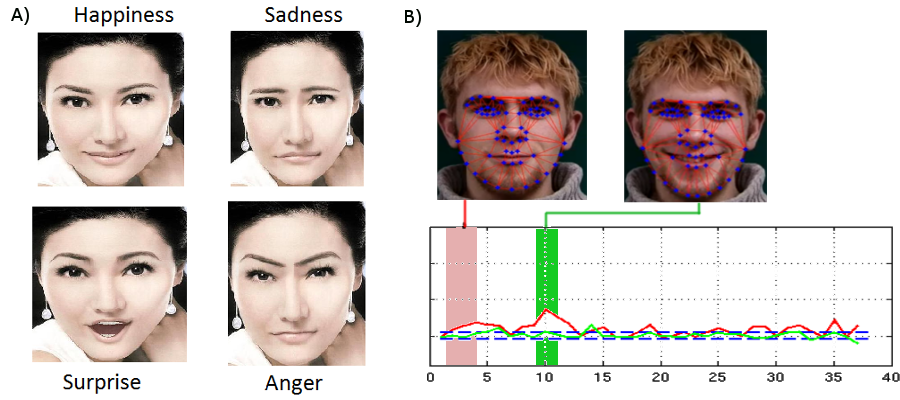
\includegraphics[scale=0.4]{images/emotionsAndGraphics1.png}
    \caption[Basic human emotions and Facial gesture analysis]{(A) Basic human emotions. (B) Facial gesture analysis. Emotion is a complex psychophysiological experience of an individual's state of mind as interacting with biochemical (internal) and environmental (external) influences}
    \label{fig:BasicEmotions}
\end{figure}

In computer vision and artificial intelligence (AI) there are many sub-problems related to facial emotion recognition such as: pose variations, people constantly moving their head in different angles; illumination changes, different environments with different illumination conditions; occlusion, which occurs when an object is in front of the face difficulting the analysis feature extraction task; background complexity, multiple objects in the environment with non-uniform background contrast; finally, image resolution which affects the accuracy of the tracking/recognition process. Besides, from the computational point of view, this problem implies the classification of facial motion or facial structure deformation into abstract representations completely based on visual information.

\subsubsection{Basic concepts}

Computational facial analysis methods can be classified in deformation extraction methods and motion extraction methods \cite{Fasel01}:
\begin{description}
\item[Motion extraction:] these approaches focus on facial changes presented as consequence of facial expressions.
\item[Deformation extraction:] these approaches work with a neutral face images or face models for extract relevant facial features not caused by wrinkles or accidents.
\end{description}

The main difference between them is that deformation-based methods can be applied to image sequences, in the second case, the analysis can be applied to both single images and image sequences by processing frames independently. However, deformation-based feature extractors miss low-level directional motion information, i.e. they cannot reconstruct pixel motion. Although face motion can be inferred by using facial feature models it requires extra computation time to achieve it.

In both cases, facial features may be processed holistically (the faces are analyzed as a whole) or locally (focusing on features from specific areas).These approaches are focused on the extraction and analysis of two types of facial features \cite{Fasel01}:
\begin{description}
\item[Intransient facial features:] always are in the face and could be deformed by facial expressions, for example, eyes, eyebrows and mouth.
\item[Transient facial features:] consider wrinkles and bulges in the face, for example, when the people open and close their eyes or mouth, face changes.
\end{description}

In both cases, the success of the technique depends on the capacity to segment the face from background. The correct segmentation allows an accurate extraction of points of interest from the faces. To do it, facial processing may take place either holistically, or locally, by focusing on facial features or areas that are prone to change with facial expressions. The task of separating the face from the background is done through segmentation, which allows the isolation of transient and intransient features within the face, that can be used to separate faces of interest from the background.

\subsubsection{Facial gestures analysis methods}
Facial gesture analysis is a challenging task and it has several application related to human interaction and computers. Traditionally, facial gestures recognition classifies the expressions into seven general emotions (anger, happiness, fear, sadness, contempt, disgust, surprise), in contrast, the facial expression analysis involves the reconstruction of facial motion, considering this way the facial muscle periods of motion between one gesture and another. In this cases it is necessary a robust classification and tracking technique of face gestures and head position \cite{Cinar01}.

There are three main steps for working in facial gestures recognition: face detection, extraction of facial gestures information and classification of the information extracted. As it was previously stated, the methods for facial gesture analysis can be grouped in deformation extraction and motion extraction.% (see Tables \ref{tb:Deformation} and \ref{tb:Motion}).

\begin{comment}
\subsubsection{Deformation extraction}
This type of methods are characterized by shape and texture changes and tendency to high spatial gradients that are good indicators for facial actions and may be analyzed either in the image or the spatial frequency domain.
The latter can be computed by techniques like Gabor wavelet-based filters, which closely model the receptive field properties of cells in the primary visual cortex \cite{Daugman1}.

These techniques are divided in three groups:

\begin{itemize}
\item Holistic image-based approaches.There are a considerable number of authors that have worked with whole faces as features. Most of them use 2D images as input so they cannot infer depth-based information. For example, some researches have been inspired in the behavior of the simple cells in the visual cortex and they model the face with Gabor wavelets \cite{Choi}. %This method present better results in many aspects from earlier work \cite{Xiaohua2009, Lai2005}.
\item Holistic Model-based approaches. Are an alternative to image-based deformation extraction. The main characteristic of these types of methods are that allow separate and process different information sources like illumination and deformation changes. Faces are analyzed by two different approaches: Active Shape Model (ASM) \cite{Wan01} and Active Appearance Model (AAM)%\cite{Lee2009}
, this helps to determinate shape, scale and pose by fitting an appropriate point distribution model to the object of interest. Other authors have decided combine Gabor filters and AAM, as a result, this techniques can lead to more accurate matching when condition changes \cite{Gao}.
\item Local image-based approach. These techniques extract facial features from windows placed around regions of the face (one or both eyes, mouth, etc.) and are used for analysis or specific purposes. New strategies are being developed
%\cite{Zhang01, Abate2007}
, for example, face recognition based on the multi-scale local structures of the face \cite{Geng01} image where the focus is in contribute to all major steps in the feature extraction and image matching, this strategy search for the nearest subject and a two-stage image matching scheme are developed for the face identification task.
\end{itemize}

%-------------------------------------------------- TABLE 1 -----------------------------------------------------------------------------------------
\begin{table}[h]
\scriptsize
%\footnotesize
\begin{center}

\begin{tabular}{|p{4.0cm}|p{4.0cm}|p{4.0cm}|} \hline \hline
\normalsize{\bf Deformation extraction} & \normalsize{\bf Holistic methods} & \normalsize{\bf Local Methods} \\  \hline \hline
\normalsize{ Image-Based}  &  \normalsize{Gabor wavelets \cite{Kruger2002}}   & \normalsize{Multi\-scale local image structures \cite{Geng01}} \\ \hline
\normalsize{ Model-based } &  \normalsize{Active Appearance Model \cite{Cootes2002}} & \\ \hline \hline
\end{tabular}
\end{center}
\caption{Holistic and local methods for deformation extraction}
\label{tb:Deformation}
\end{table}

It is important to remark that most of the techniques found in this category uses 2D images as input. Some techniques uses explicit geometry of the face to reconstruct it or to infer depth (AAM).

\subsubsection{Motion Extraction}
These types of methods have been commonly used for the task of facial expressions analysis extracting features of the face of images sequences;there are applications about it, for example in surveillance, motion capture, image stabilization or feature tracking for 3D reconstruction.

\begin{itemize}
\item Holistic dense optical flow. Is used when is necessary analyze whole faces, when is presented motion of objects. This type of techniques can be in real time or non-real time using video databases. Other techniques implement dense optical flow map \cite{Tagliasacchi2007} trying to be more efficient, fast and making use of the minimum computational cost. 3D optical flow models is other technique and  is derived from a straightforward extension of the 2D Horn–Schunck model and discretized using standard finite differences. %\cite{elMostafa}.
\item Holistic motion models.A 3D model is used mainly to be precise to enhance the facial expression recognition or face recognition. Markov models are widely employed to recognize faces or expressions  \cite{Wang01}. Kalman filter is important in this type of techniques due to its ease and accuracy in motion and recognition of objects, in this case, faces and expressions.% \cite{Motai2012}.
\item Local motion models. Over the last years, 3D face models have been widely used in many applications, for example, face recognition, facial animation and facial expression analysis. 3D Morphable model(MMs) have become a popular tool to build and fit 3D face models to images \cite{mora}.%, Levine2009}.
\item Feature point tracking.In this techniques, motion estimates are obtained when a set of features are  selected of the face (lips, nose, eyes, etc.) Is important to note, in this techniques is important that environment is clear and have good illumination, those factors between others reduce the risk of tracking loss. There are strategies that present a different approaches about that, showing a drift-correcting template update trying to have more precision for tracking a feature point in 2D \cite{Peng}. This method has a more sustained ability to track a feature point than other previous strategies.
\end{itemize}

%-------------------------------------------------- TABLE 2 -----------------------------------------------------------------------------------------
\begin{table}[h]
\scriptsize
%\footnotesize
\begin{center}

\begin{tabular}{|p{4.0cm}|p{4.0cm}|p{4.0cm}|} \hline \hline
\normalsize{\bf Motion extraction} & \normalsize{\bf Holistic methods} & \normalsize{\bf Local methods} \\  \hline \hline
\normalsize{Dense optical flow}  &  \normalsize{Dense flow fields \cite{Holte01}}  & \normalsize{Flow-based facial expression \cite{Sanchez01}}  \\ \hline
\normalsize{Motion models}  &  \normalsize{3D motion models \cite{Urtasun2006}} & \normalsize{3D Morphable Model \cite{Vetter01}} \\ \hline \hline
\normalsize{Feature point tracking}  &   & \normalsize{Eigenface augmented \cite{Yuki01}} \\ \hline \hline
\normalsize{Difference-images}  &  \normalsize{Holistic diff. images \cite{GarciaMartinez2012}} &  \\ \hline \hline
\end{tabular}
\end{center}
\caption{Holistic and local methods for motion extraction}
\label{tb:Motion}
\end{table}
\end{comment}

\subsubsection{Review of Deformation and Motion Extraction Methods}
Over last years researchers have developed many approaches and models for face recognition and analysis with good results by using both deformation and motion extraction approaches. Although, the election of an specific technique relies on the characteristics of a certain problem. Deformation extraction have been successfully used to solve emotion recognition tasks, since they can be used to analyze single images. However, if the problem consists in analyzing a sequence of images to extract the \emph{motion} (caused by muscles actions) of different regions in the face while making a gesture, the motion extraction techniques are ideal to this goal, since they have been applied to evaluate the motion produced in areas like eyes or mouth, by using a model generated a priori.

In general, motion techniques uses either 2D or 3D information. Typically, 2D based techniques are more used due to their fastness, product of a reduced dimensionality of the information. Nevertheless,  a very large training data sets is needed to model the angular variations and illumination changes. In the case of 3D based approaches, the accuracy reached is higher than 2D based ones \cite{Fang2012}, since they are rotation invariant, although their sensitiveness to illumination changes remains.% \cite{Stratou2011}.

In the case of facial expression analysis, precision is more important than processing speed, since the analysis can be carried on offline. Considering that, 3D based techniques are more relevant to solve the problem; especially those approaches with local oriented processing, since they allow analyzing information from specific points in the face (opposed points in the face are required in order to analyze the symmetry).

% The table from 3d/4d methods doesn't specify the origin from the databases
\subsubsection{3D based local analysis techniques}
As it was previously stated, the main difference about these techniques is the way they process information. Holistic approaches considers the whole image to extract motion vectors, which could be used for extracting general information about the motion of the face; still to increase the accuracy of facial expressions analysis requires the motion interpretation of specific regions in the face. On this line, there are several techniques in the state of the art (see Table \ref{tb:3DLocalTechniques}) that focuses on specific regions in the face:

\begin{table}[h]
\scriptsize
%\footnotesize
\begin{center}
\begin{tabular}{||p{2.7cm}|p{2.0cm}|p{2.0cm}|p{2.0cm}|p{1.5cm}|p{1.5cm}|p{1.5cm}||} \hline \hline
Reference & Sequences & Landmarks & Database & Expr. Types & R.P. (\%) \\ \hline \hline
\normalsize{Yin \cite{Yin2006}} & 2D + 4D & 64 semi-auto & BU-3DFE & 6 & 80.2 \\ \hline \hline
\normalsize{Wang \cite{Wang2007}} & 2D + 3D & 58 auto & Private & 4 & 83.0 \\ \hline \hline
\normalsize{Sun \cite{SunFer2008}} & 2D + 4D & 83 auto & BU-4DFE & 6 & 80.9 \\ \hline \hline
\normalsize{Rosato \cite{Rosato2008}} & 2D + 4D & 22 auto & BU-3DFE, BU-4DFE & 7 & 80.1 \\ \hline \hline
\normalsize{Zhao \cite{Zhao01}} & 2D + 3D & 19 manual & Bosphorus & 7 & 94.2 \\ \hline \hline
\normalsize{Tsalakanidou \cite{Tsalakanidou2010}} & 2D + 4D & 81 auto & Private & 5 & 85.0 \\ \hline \hline
\end{tabular}
\end{center}
\caption[Methods for $3D/4D$ Facial Expression Analysis]{Methods for $3D/4D$ Facial Expression Analysis (\footnotesize{Headers: \textbf{Sequences} denotes the dimensions of the images where 2D denotes whether the method makes use of the 2D texture associated with the 3D data and 4D denotes whether the method uses temporal information from a sequence of 3D data; \textbf{Database} denotes the database from which a subset was selected; \textbf{R.P.} denotes reported performance, which is the average recognition rates}).}
\label{tb:3DLocalTechniques}
\end{table}

\begin{comment}
\begin{itemize}
\item Sun et al. \cite{SunFer2008} designed a methodology for facial expression recognition (FER) considering 3D images. They propose a spatio-temporal expression analysis approach based on a new modality, 3D dynamic geometric facial model sequences, to tackle the FER problems. This approach integrates a 3D facial surface descriptor and Hidden Markov Models (HMM) to recognize facial expressions. To study the dynamics of 3D dynamic models for FER, have been investigated three types of HMMs: temporal 1D-HMM, pseudo 2D-HMM (a combination of a spatial HMM and a temporal HMM), and real 2D-HMM.

\item Rosato et al. \cite{Rosato2008} developed an effective approach to automatically establish vertex correspondences for feature registration, and further classify facial models to specific expressions in 3D facial images. Their technique also has the hability for 3D facial expression labeling, registration, tracking, and categorization. According to the authors, one of the major obstacles for analyzing such data is lack of correspondences of features (or vertices) due to the variable number of vertices across individual models or 3D model sequences. In this work they also describe a 3D facial expression databases created with 3D facial range models of the face created with static range scanners.

\item Tsalakanidou et al \cite{Tsalakanidou2010} developed a technique for automated facial action and facial expression recognition system using 2D+3D images recorded in real-time by a structured light sensor. It is based on local feature tracking and rule-based classification of geometric, appearance and surface curvature measurements. Also conducted some experimentos under relatively non-controlled conditions demonstrate the accuracy and robustness of the approach.

\item Yin et al. \cite{Yin2006} developed an automatic techniques for 3D expression model analysis by tracking and classification mechanisms. For this, they analyze the face surface as a three dimensional timevarying 'wave', which is associated with the movement of facial expressions. They found that by tracing the behavior of the 3D primitive features precious information about the nature of the underlying physical process could be revealed. This investigation propose to study the intensity-variant facial expressions in a 3D space.

\item  Wang et al. \cite{Wang2007} developed a methodology for analyzing the facial images of schizophrenic patients by combining 2D and 3D information. The main difficulty of this type of patients is that they usually have impaired expressions in the form of 'flat' or inappropiate affects, which make the quantification of their facial expressions a challenging problem. To solve this problem the authors propose the extraction of features that includes 2D and 3D geometric features, and the moment invariants combining both 3D geometry and 2D textures.

\item Zhao et al.  \cite{Zhao01} proposed a methodology for extracting the facial action units (specific deformable regions in the face like the nostrils). Action units deform facial appearance simultaneously in landmark locations and local texture as well as geometry on 3D faces, so it is necessary to extract features from multiple facial modalities to characterize these deformations comprehensively. In order to fuse the contribution of the discriminative power from all features efficiently, authors propose to use a extended statistical facial feature models (SFAM) to generate feature instances corresponding to AU class for each feature. Then the similarity between each feature on a face and its instances are evaluated so that a set of similarity scores are obtained.
\end{itemize}

Albeit some authors that opted to create their own data bases of images/sequences there are some public data bases that offers a good reference point to evaluate the performance of our application, some of them are shown in table \ref{tb:Databases}:

\begin{table}[h]
%\scriptsize
\footnotesize
\begin{center}
\begin{tabular}{||p{2.7cm}|p{2.0cm}|p{2.0cm}|p{2.0cm}|p{1.5cm}|p{1.5cm}||} \hline \hline
Database & Subjects & Samples per subject & Total images & Expressions & Poses \\ \hline \hline
\normalsize{BU-3DFE  \cite{Lijun2006}} & 100 & 25 & 2500 & 6 expressions & n/a \\ \hline \hline
\normalsize{BU-4DFE \cite{Lijun2006}}& 101 & 6 & 606 & 6 expressions & n/a \\ \hline \hline
\normalsize{Bosphorus \cite{Savran2008}} & 105 & 31-54 & 4652 & 6 expressions & 13 pitch, yaw, and cross rotations \\ \hline \hline
\normalsize{York-3DFace \cite{Heseltine2008}} & 350 & 15 & 5250 & 5 expressions & Uncontrol led up and down \\ \hline \hline
\end{tabular}
\end{center}
\caption[Public images databases]{Public images databases and their statistics}
\label{tb:Databases}
\end{table}

\end{comment}

The approaches described previously have the ability to perform facial expressions analysis considering 3D information. This techniques can be classified into two main groups, depending on the labelling mechanism: automatic and manual. In the case of the automatic labelling mechanisms, authors have used automatic fitting techniques to extract different numbers of facial regions of interest (22- \cite{Rosato2008} and 58 \cite{Wang2007}). In the case of the manual labelling mechanisms, the existing techniques require off line characterization of the facial regions of interest. As it can be seen in Table \ref{tb:3DLocalTechniques}, there is a difference on the percentage of recognition achieved by techniques in these two categories: methodologies designed to manual labelling reached as top a 94.2\% compared to 85.0\%. Also from the table \ref{tb:3DLocalTechniques}, there is no clear difference about the number of points to be used (but the higher the number of points is the higher computational complexity as well as a higher recognition rate). Although it remains to review, automatic labelling techniques are more desirable for facial expression analysis problems, since they reduce the dependance from user interaction.
%Even though there are some functional commercial applications they need to stablish some restrictions to obtain higher recognition rates and are more oriented to emotion recognition rather than facial expression analysis, as it can be seen in the following.

\begin{comment}

\subsection{Commercial software}
\label{Sec:ComSoft}

There are different software for facial expression recognition, but none is 100\% effective. One of them is {\bf faceAPI \cite{faceApi2}} that allows  to incorporate Seeing Machines world class face tracking technology into one product or application. faceAPI provides a suite of image-processing modules created specifically for tracking and understanding faces and facial features. Seeing Machines faceAPI is the only comprehensive, integrated solution for developing products that leverage real-time face tracking. All image-processing for face tracking is handled internally, removing the need for any computer vision experience. \\

The features of this software are:
\begin{itemize}
\item Highly robust, real-time, automatic monocular 3D face tracking.
\item Tracks head-position in 3D providing X,Y,Z position and orientation coordinates per frame of video.
\item Tracks 3 points on each eyebrow and 8 points around the lips.
\item Pose-normalized face texture output, annotated with facial feature coordinates.
\item Can track up to +/- 90 degrees of head rotation.
\item Robust to fast movements, large head rotations, lighting, facial deformation, skin color, beards, glasses etc.
\end{itemize}

\begin{figure}[H]
    \centering
    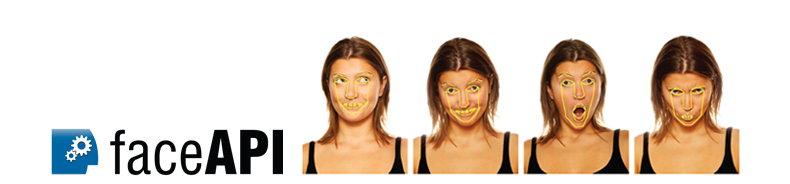
\includegraphics[scale=0.5]{faceapi.png}
    \caption{faceApi software.}
    \label{fig:faceApi software}
\end{figure}

{\bf Affdex} \cite{affdex2}is other commercial software for facial expressions recognition. Affdex reads emotional states such as surprise, dislike and attention from facial expressions using a web cam. It employs advanced computer vision and machine learning techniques to recognize and automate the analysis of tacit expressions, and it applies scientific methods to interpret viewers' emotional responses quickly and at scale. \\

The main features of this software are:
\begin{itemize}
\item Affdex integrates seamlessly into an existing survey process from measurement through insight. This includes the Affdex dashboard, where survey results are combined with Affdex emotional analysis for more power insights, faster.
\item Affdex unleashes the power of cloud computing coupled with a simple web cam to easily and cost-effectively reach more people, in more places.
\item Automatic segmentation analysis through survey integration.
\end{itemize}

\begin{figure}[h]
    \centering
    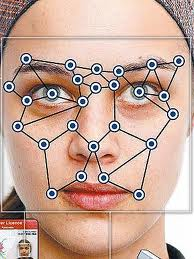
\includegraphics[scale=0.5]{facialExpression1.jpg}
    \caption{Affdex software.}
    \label{fig:Affdex software}
\end{figure}

Though, there disadvantages in this type of software, for example:
\begin{itemize}
\item They are not tolerant to occlusion.
\item Their accuracy decreases when illumination is low.
\item They can not determine whether the emotion is feigned.
\item they only can recognize specific expressions, cannot be trained.
\end{itemize}


Considering the reviewed information about different techniques for human facial expression analysis we state the problem and research questions in the next section.
\end{comment}

\section{Neural Networks}
	The study of facial gestures has acquired an increasing interest since it has a huge application area. Facial gestures can be defined as a movement produced in the face by muscles while contracting (see Figure \ref{fig:Facial muscles}) with the objective to transmit thoughts or emotions, for example when a person communicates with others. The interpretation of non-verbal human communication, like facial gesticulation during a talk, is a very common activity and is done intrinsically. Equally important is the interpretation of gestures, through this, people can improve their interpersonal understanding. For example, by analyzing the mood of a speaker it is possible to confirm the intention of a message.

\begin{figure}[ht]
\centering
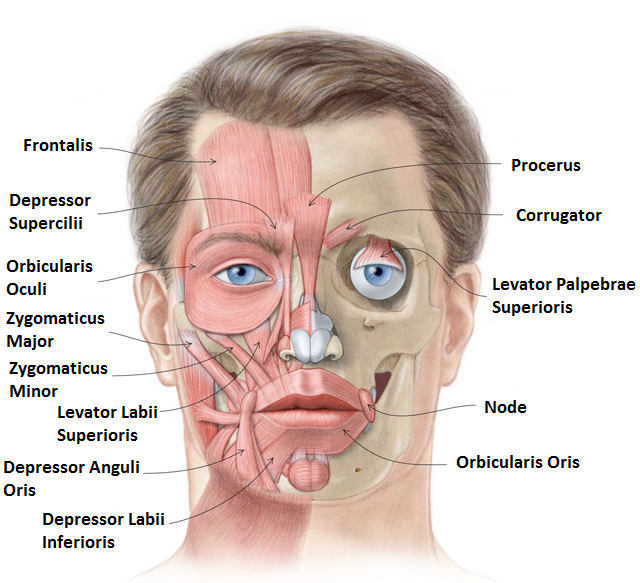
\includegraphics[scale=0.5]{images/Figure11FacialMuscles_name_2.png}
\caption{Facial muscles}
\label{fig:Facial muscles}
\end{figure}

Traditionally, computational applications have tried to interpret emotion by associating a facial image to one of the seven general expressions (such as fear, anger, happiness, etc) but they are too general and they do not evaluate the symmetry of the emotion. This can be solved considering the psychological perspective of the emotions. According to Ekman \cite{Hager1979} the symmetry of a gesticulation can describe the veracity of a expression. The bases for this are some studies of the amygdala, which is a region in the brain (located in the medial temporal lobes) that performs the analysis of expressions.

However, this task is complex, since involves temporal processing of muscles contractions. To approach this problem, one can look at biological systems that perform this analysis accurately. An example of this is the human brain, which can perform the analysis even under varying environment conditions like: illumination changes, occlusion and pose changes. This is a motivation for the developing of bio-inspired systems based on the behavior of the amygdala, more precisely modeling the neuron interaction for analysis facial motion produced by the gestures.

From all the involved parts gesture eye gaze is the most important element since it express sincerity and credibility. Together, all the elements of facial muscles can transmit the feelings of the speaker, from happiness, to depth concern. This was previously affirmed by Darwin (1872), who stated that facial gesticulation for emotion transmition is innate and very similar for all people, since we evolved very similarly. His theory was not accepted before due to some detractors like Bruner et al. (Bruner \& Tagiuri, 1954). Later, Ekman et al. \cite{Hager1979} solved this issue definitively by pointing out methodological problems that had confused other researchers. They showed that observers could agree on how to label both posed and spontaneous facial expressions in terms of either emotional categories or emotional dimensions. Much evidence, including reanalysis of negative studies, indicated that facial expressions can provide accurate information about emotion.

Therefore the analysis of facial expressions constitutes a critical and complex portion of our non-verbal social interactions. Over the past years there has been an increasing interest on developing automated computational tools for facial expression analysis.

\begin{comment}
However, the automatic facial expression analysis is a complex task, on one hand face structure distribution is different from one individual to another. On the other, faces are analyzed from sequences of images captured in environments with variations (such as lighting, pose and scale changes) that difficult the extraction of this structure. From the computational point of view, this problem implies the classification of facial motion and facial structure deformation into abstract representations completely based on visual information.
\end{comment}

To address this analysis it is necessary to perform two main tasks: face acquisition and facial feature extraction. In the first one, techniques have been developed to deal with the extraction and normalization of the face considering variations in the pose %\cite{Essa1997, Rowley1998} 
and illumination. %\cite{Fellenz1999, Belhumeur1997}. 
However, most of the effort has focused to the feature extraction issue~\cite{Fasel2003}, since techniques like appearance-based model %\cite{Lanitis1997, Kim2004, RuizdelSolar2008} 
try to deal with significant variations in the acquired face images without relying on normalization.

\begin{figure}[ht]
    \centering
    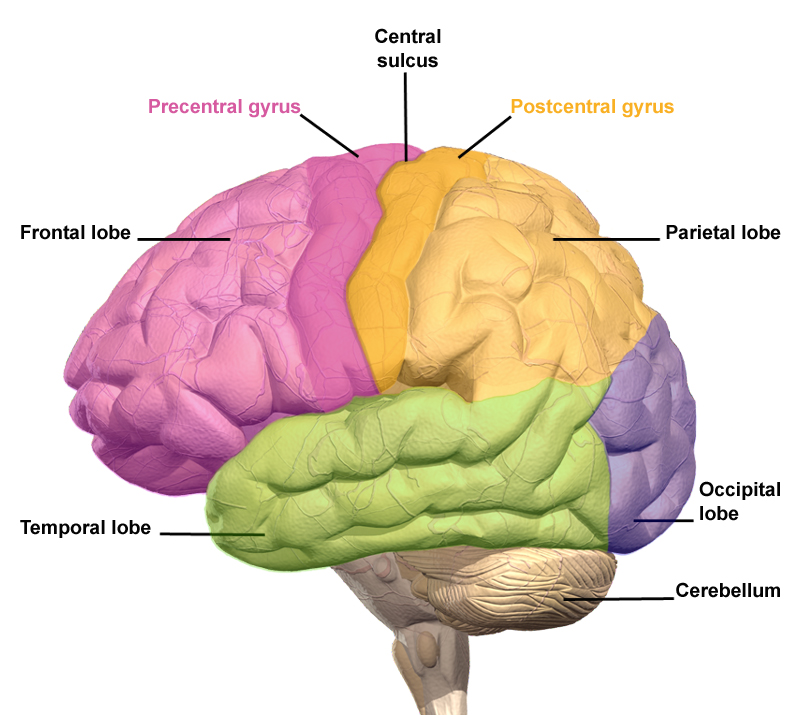
\includegraphics[scale=1.0]{images/Figure6Brain.png}
    \caption{Brain anatomy}
    \label{fig:Brain anatomy}
\end{figure}

The analysis problem has been approached from two main streams~\cite{Fasel2003}: facial deformation extraction models and facial motion extraction models. Motion extraction approaches directly focus on facial changes produced by facial expressions, whereas deformation-based methods contrast the visual information against face models to extract features product of expressions and not by age deformation like wrinkles.

\begin{comment}
In the case of deformation methods the extraction of features relies on shape and texture changes through a period of time. On one hand the holistic approaches either use the whole face \cite{JyostnaDevi2010}%, Nair2011} 
or partial information about regions in the face like mouth or eyes \cite{Gu2012}.%, Venkatesh2009, Maalej2011}. 
In the case of the motion extraction, the features are extracted by analyzing motion vectors, again this can be done holistically %\cite{Dornaika2011, Sanchez2011}
, and locally.%\cite{Park2009, Xiang2008, Wang2009}.
\end{comment}

Another approach to solve this problem, is by looking at biological systems that perform accurately this task. The human brain can analyze the information from the face using an area called amygdala \cite{Sergerie2008} (an area located in the medial temporal lobes) which receives connections from other areas like visual cortex. How exactly the amygdala works remains unknown; however, it is know that this area sends impulses to the hypothalamus for activation of the sympathetic nervous system, to the thalamic reticular nucleus for increased reflexes, to the nuclei of the trigeminal nerve and the facial nerve, and to the ventral tegmental area, locus coeruleus, and laterodorsal tegmental nucleus for activation of dopamine, norepinephrine and epinephrine.% \cite{Amunts2005}.

The cortical nucleus is involved in the sense of smell and pheromone-processing. It receives input from the olfactory bulb and olfactory cortex. The lateral amygdala, which send impulses to the rest of the basolateral complexes and to the centromedial nuclei, receive input from the sensory systems. The centromedial nuclei are the main outputs for the basolateral complexes, and are involved in emotional arousal in rats and cats. Several studies confirm that the amygdala receives inputs from visual cortex when it comes to emotion processing. Lateralization of processing visual information in the amygdala might indicate symmetry analysis activity which was first found by Ekman et al \cite{Hager1979}. In their studies they found that emotion understanding is directly related to symmetrical analysis of opposed facial regions.

This information is relevant since provides hints on the role of the amygdala during the expression of emotions and visual interpretation of them. How the visual information is processed remains unclear, but it is known that the information is processed laterally (information is processed in one hemisphere). This can be used as a source of inspiration to build a neural architecture that allows processing opposed facial regions to interpretate emotions. Previously some researchers have used traditional neural networks (NN) to recognize emotions from face images\cite{Spiros2005}%, MatsuguKatsuhiko2003, MuhammadPrevost2008}
; however, NN in those works are used for recognition purposes though symmetry understanding in facial gestures requires analyzing the evolution of muscles during gesticulation rather than just comparing gesture moments. This means that not all neural networks models are adequate for this task, in fact NN approaches can be classified in 3 generations, the two first are usually related to recognition tasks while the third also allows temporal information processing.

\subsubsection{Generations of Neural Networks}
Over the past hundred years, research has accumulated knowledge about the structure and function of the brain. The elementary processing units in the central nervous system are neurons which are connected to each other in an intricate pattern. Examples of this types of neurons are sketched in Figure \ref{fig:NeuronTypes} which shows a drawing by Ram\'on y Cajal, one of the pioneers of neuroscience around 1900. In his work, he distinguished several types of neurons, with different physical structures like triangular or circular. This picture gives a glimpse of the network of neurons in the cortex. In fact, cortical neurons and their connections are packed into a dense network with more than 104 cell bodies and several kilometers of ``wires'' per cubic millimeter. In all areas, however, neurons of different sizes and shapes form the basic elements. Wolfgang Maass (Maass, 1997) outline past and current artificial neural network research into three generations and made the following observations~\cite{Maass1996}.

\begin{figure}[ht]
    \centering
    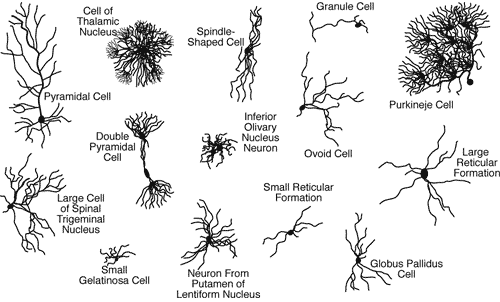
\includegraphics[scale=0.7]{images/Figure1Neuron_Types.png}
    \caption[Types of neurons]{\small{There are three kinds of neurons: motor neurons (for conveying motor information), sensory neurons (for conveying sensory information), and interneurons (which convey information between different types of neurons). The image identifies how neurons come in various shapes and sizes.}}
    \label{fig:NeuronTypes}
\end{figure}

A typical neuron can be divided into three functional parts called: dendrites, soma, and axon (see Figure \ref{fig:NeuronStructure}). Roughly speaking, the dendrites play the role of the ``input device'' that collects signals from other neurons and transmits them to the soma. The soma is the ``central processing unit'' that performs an important non-linear processing step: If the total input exceeds a certain threshold, then an output signal is generated. The output signal is taken over by the ``output device'', the axon, which delivers the signal to other neurons.

The junction between two neurons is called a synapse. Let us suppose that a neuron sends a signal across a synapse, the sender is called presynaptic cell and the receiver is called postsynaptic cell. A single neuron in vertebrate cortex often connects to more than $10^4$ postsynaptic neurons. Many of its axonal branches end in the direct neighborhood of the neuron, but the axon can also stretch over several centimeters so as to reach to neurons in other areas of the brain.

In the literature there are different computational models that intent to simulate the behavior of these neurons communities. Roughly, they can be divided in three generations, considering their chronological appearance order. Our attention is centered in the third generation since it allows temporal processing of input patterns.

The \textbf{first generation} is based on the McCulloch-Pitts neuron (also known as a perceptron or a threshold-gate) as the basic computation unit. Models of the first generation, such as the multi-layer perceptron, use digital input and output, usually binary or bipolar. The perceptron is a type of artificial neural network (ANN) invented in 1957 at the Cornell Aeronautical Laboratory by Frank Rosenblatt~\cite{Rosenblatt1960}.

The \textbf{second generation} is based on computation units (neurons) that use an activation function of a continuous set of possible output values.% Commonly, these activation functions are the sigmoid, $f(x) = 1 / 1 + e^{- \sigma x}$, or the hyperbolic tangent, $f(x) = (1 - e^{-2x}) / (1 + e^{-2x})$. 
This generation, like first one, can compute arbitrary boolean functions (after using a threshold). Also, a concept of hidden layer appeared, through it more complex functions can be approximated~\cite{Rosenblatt1962}. Important to many implementations is the fact that second generation networks support learning algorithms based on gradient descent, such as error back-propagation.

\begin{figure}[ht]
    \centering
    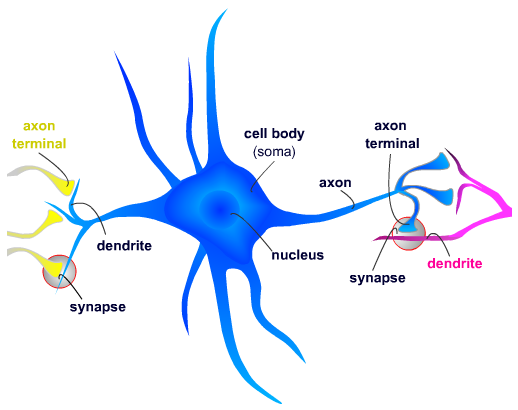
\includegraphics[scale=0.6]{images/Figure2NeuronStructure.png}
    \caption{Structure of a neuron}
    \label{fig:NeuronStructure}
\end{figure}

The \textbf{third generation} is known as Spiking Neural Networks (SNN) model. They increase the level of realism in a neural simulation, in addition to neuronal and synaptic states. The SNNs also incorporate the concept of time into their operating model, the idea is that neurons in the SNN model do not fire at each propagation cycle (as it happens with typical multi-layer perceptron networks), but rather fire only when a membrane potential\footnote{an intrinsic quality of the neuron related to its membrane electrical charge} reaches a threshold. When a neuron fires generates a signal that travels to other neurons that are stimulated (excited or inhibited) by this signal. In the context of spiking neural networks, the current activation level (modeled as some differential equation) is normally considered to be the state of the neuron, with incoming spikes pushing this value higher, and then either firing or decaying over time. Various coding methods exist for interpreting the outgoing spike train as a real-value number, either relying on the frequency of spikes, or the timing between spikes, to encode information.

\begin{figure}[ht]
    \centering
    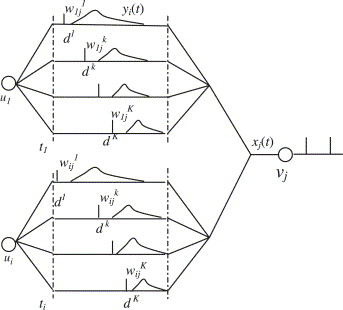
\includegraphics[scale=4.0]{images/Figure10SNN.png}
    \caption{Spiking Neural Network}
    \label{fig:Spiking Neural Network}
\end{figure}

These networks, like multi-layer perceptron networks, can approximate continuous arbitrary functions, as well as, temporal encoded inputs and outputs (\cite{Maass1996}).  This kind of neural network, in principle, can be used for information processing applications the same way as traditional artificial neural networks. However, due to their more realistic properties, they can also be used to study the operation of biological neural circuits. Some successful models of SNNs have been used to solve real-life problems, such as, navigation in mobile communities of robots \cite{WangHouZou2008}.%, BatlloriLaramee2011}. Another interesting field is sounds processing, where the SNNs have been used to detect the source of a sound \cite{NaldaCases2008}.

\begin{comment}
\subsection{SNN models}
Below there is review some widely used models of spiking and bursting neurons that can be expressed in the form of ordinary differential equations (ODE). It considers whether the models have biophysically meaningful and measurable parameters, and whether they can exhibit autonomous chaotic activity. Throughout this section, $v$ denotes the membrane potential and $v'$ denotes its derivative with respect to time. All the parameters in the models are chosen so that $v$ has $mV$ scale and the time has $ms$ scale. To compare computational cost, it is assumed that each model, written as a dynamical system $ x = f(x) $, is implemented using a fixed-step first-order Euler method $x(t+ \tau )=x(t)+ \tau f(x(t))$ with the integration time step chosen to achieve a reasonable numerical accuracy.

The models reviewed, have the computational ability of mimic various biological behaviors of neurons when they are stimulated by the incoming pulses, biological features like: excitability (tonic spiking), single spike at the onset of the input (phasic spiking), periodic bursts of spikes (tonic bursting), burst transmitting at beginning stimulation (phasic burst), bursting then spiking (mixed model), tonic spike with decreasing frequency (spike frequency adaptation) for mention a couple of them. All these characteristics of the action potential are represented, between other, by the three models which we are going to review next. Also these models have a low cost computational (number of floating point operations FLOPS).

There is a focus on three SNN models because they are very biologically plausible and they represent a low implementacion. The models are:

\begin{itemize}
\item Integrate-and-Fire-or-Burst
\item Resonate-and-Fire
\item Spiking Model by Izhikevich~\cite{Izhikevich2003}
\end{itemize}
\vspace{0.5cm}

\textbf{Integrate-and-Fire-or-Burst}\\
Smith and coauthors \cite{SmithRinzel2000} suggested an improvement integrate-and-fire-or-burst (I\&FB) to model thalamo-cortical neurons.

$$
\begin{array}{lr}
v'  =  I+a-bv+gH(v-v_h)h(v_T-v) \\
\mbox{if} \hspace{0.3cm} v  =  v_{tresh}, \hspace{0.5cm} \mbox{then} \hspace{0.2cm} v \leftarrow c \\
h'=
\left\{
\begin{array}{lr}
\frac{-h}{\tau^-}, \hspace{1cm} \mbox{if} \enspace v > v_h \\
\frac{(1-h)}{\tau^+}, \hspace{1cm} \mbox{if} \enspace v < v_h
\end{array}
\right.
\end{array}
$$

where $h$ describes the inactivation of the calcium $T$-current $g,v_h,v_T,\tau^+$ and $\tau^-$ are parameters describing dynamics of the $T$-current, and $H$ is the Heaviside step function. Having this kind of a second variable creates the possibility for bursting and other interesting regimes summarized in Table \ref{tb:ModelsComparison}. But this comes with a price: It takes between 9 and 13 operations (depending on the value of $v$) to simulate $1 ms$ of the model.

\textbf{Resonate-and-Fire}\\
The resonate-and-fire neuron \cite{Izhikevich2001} is a two-dimensional (2-D) analogue of the I\&F neuron.

$$
\begin{array}{lr}
z'=I+(b+iw)z\\
\mbox{if} \enspace Imz=a_{tresh}, \quad \mbox{then} z\leftarrow z_0(z)
\end{array}
$$

where the real part of the complex variable $z$ is the membrane potential. Here $b,w$ and $a_{tresh}$ are parameters, and $z_0(z)$ is an arbitrary function describing activity-dependent after-spike reset. The resonate-and-fire model is simple and efficient -it takes $10$ operations to simulate $1 ms$. When the frequency of oscillation $w=0$, it becomes an integrator. Its neuro-computational properties are summarized in Table \ref{tb:ModelsComparison}.

\textbf{Spiking Model by Izhikevich (2003)}\\

A simple model of spiking neurons proposed recently by Izhikevich \cite{Izhikevich2003}.

\begin{eqnarray}
\label{eq:1}
v' & = & 0.04v^2+5v+140-u+I \\
u' & = & a(bv-u)
\end{eqnarray}

with the auxiliary after-spike resetting.

\begin{eqnarray}
\label{eq:2}
\mbox{if} \enspace v \ge +30\mbox{mV}, \quad 
\mbox{then}
\left\{
\begin{array}{lr}
\label{eq:3}
v \leftarrow c \\
u \leftarrow u+d
\end{array}
\right.
\end{eqnarray}

where $v$ represents the membrane potential of the neuron and $u$ represents a membrane recovery variable, which accounts for the activation of $K^+$ ionic currents and inactivation of $Na ^+ $ ionic currents, and it provides negative feedback to $v$. After the spike reaches its apex ($+30 mV$), the membrane voltage and the recovery variable are reset according to this last equation. If $v$ skips over $30$, then it first is reset to $30$, and then to $c$ so that all spikes have equal magnitudes. The part $0.04v^2+5v+140$ is chosen so that $v$ has $mV$ scale and the time has $ms$ scale. Geometrical derivation of the model based on fast and slow nullclines can be found in \cite{Izhikevich2006b}.

The model can exhibit firing patterns of all known types of cortical neurons with the choice of parameters $a$, $b$, $c$, and $d$ given in \cite{Izhikevich2003}. It takes only $13$ floating point operations to simulate $1 ms$ of the model, so it is quite efficient in large-scale simulations of cortical networks. When $(a,b,c,d)=(0.2,2,-56,-16)$ and $I=-99$, the model has chaotic spiking activity, though the integration time step $\tau$ should be small to achieve adequate numerical precision.

We stress that $+30 mV$ in equation \ref{eq:3} is not a threshold, but the peak of the spike. The threshold value of the model neuron is between $-70$ and $-50$, and it is dynamic, as in biological neurons.
\end{comment}

\subsubsection{Spiking Neural Networks}
In practice, there is a major difference between the theoretical power of spiking neural networks. Some large scale neural network models have been designed to take advantage of pulse coding found in spiking neural networks. One of the most exciting characteristics of spiking neural networks (with the potential to create a step-change in our knowledge of neural computation) is that they are innately embedded in time \cite{Maass1996}.

Spike latencies, axonal conduction delays, refractory periods, neuron resonance and network oscillations all give rise to an intrinsic ability to process time-varying data in a more natural and computationally powerful way than is available to 2nd generation models. Real brains are embedded in a time-varying environment; almost all real-world data and human or animal mental processing has a temporal dimension. Evidence is growing that rhythmic brain oscillations are strongly connected to cognitive processing.% \cite{Klimesch1999, Basar2001, Engel2001, Kahana2001, Ward2003}. 
This type of processing is well suited to problems like face gesticulation characterization, since this problem implies the processing of spatial features over time periods to abstract their relations over time.

\begin{figure}[h]
    \centering
   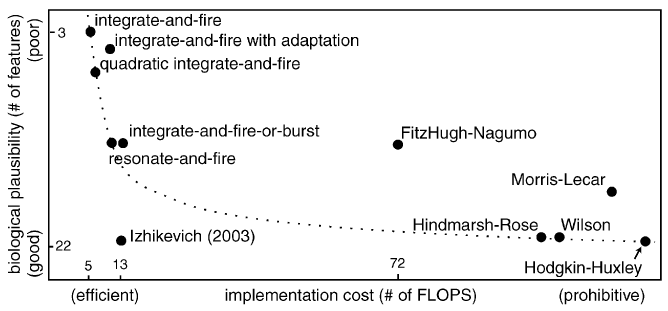
\includegraphics[scale=0.7]{images/Figure3Comparison.png}
    \caption{Comparison of spiking models: biological plausibility against implementation cost.}
    \label{fig:Comparison}
\end{figure}

\begin{comment}
\begin{table}[h]
\scriptsize
%\footnotesize
\begin{center}
\begin{tabular}{|p{3.0cm}|p{0.1cm}|p{0.1cm}|p{0.1cm}|p{0.1cm}|p{0.1cm}|p{0.1cm}|p{0.1cm}|p{0.1cm}|p{0.1cm}|p{0.1cm}|p{0.1cm}|p{0.1cm}|p{0.1cm}|p{0.1cm}|p{0.1cm}|p{0.1cm}|p{0.1cm}|p{0.1cm}|p{0.1cm}|p{0.1cm}|p{0.1cm}|p{0.1cm}|p{0.4cm}|} \hline \hline 
\bf Models & 
\multicolumn{1}{c|}
{\begin{sideways}
biophysically meaningful \
\end{sideways}} & 
{\begin{sideways}
tonic spiking \
\end{sideways}} &
{}{\begin{sideways}
phasic spiking \
\end{sideways}} &
{}{\begin{sideways}
tonic bursting \
\end{sideways}} &
{}{\begin{sideways}
phasic bursting \
\end{sideways}} &
{}{\begin{sideways}
mixed mode \
\end{sideways}} &
{}{\begin{sideways}
spike frequency adaptation \
\end{sideways}} &
{}{\begin{sideways}
class 1 excitable \
\end{sideways}} &
{}{\begin{sideways}
class 2 excitable \
\end{sideways}} &
{}{\begin{sideways}
spike latency \
\end{sideways}} &
{}{\begin{sideways}
subthreshold oscillation \
\end{sideways}} &
{}{\begin{sideways}
resonator \
\end{sideways}} &
{}{\begin{sideways}
integrator \
\end{sideways}} &
{}{\begin{sideways}
rebound spike \
\end{sideways}} &
{}{\begin{sideways}
rebound burst \
\end{sideways}} &
{}{\begin{sideways}
threshold variability \
\end{sideways}} &
{}{\begin{sideways}
bistability \
\end{sideways}} &
{}{\begin{sideways}
DAP \
\end{sideways}} &
{}{\begin{sideways}
accomodation \
\end{sideways}} &
{}{\begin{sideways}
inhibition-indiced spiking \
\end{sideways}} &
{}{\begin{sideways}
inhibition-induced bursting \
\end{sideways}} &
{}{\begin{sideways}
chaos \
\end{sideways}} &
{}{\begin{sideways}
$\sharp$ of FLOOPS \
\end{sideways}} \\  \hline \hline
\bf integrate-and-fire &  & $\bullet$  &   &  &  &  &  & $\bullet$ &  &  &  &  & $\bullet$ &   &  &  &  &  &  &  &  &  & 5 \\  \hline \hline
\bf integrate-and-fire with adaptation &  & $\bullet$ &  &  &  &  & $\bullet$ & $\bullet$ &  &  &  &  & $\bullet$ &  &  &  &  & $\bullet$ &  &  &  &  & 10 \\  \hline \hline
\bf integrate-and-fire or burst &  & $\bullet$ & $\bullet$ &  & $\bullet$ &  & $\bullet$ & $\bullet$ &  &  &  &  & $\bullet$ & $\bullet$ & $\bullet$ &  & $\bullet$ & $\bullet$ &  &  &  &  & 13 \\  \hline \hline
\bf resonate-and-fire &  & $\bullet$ & $\bullet$ &  &  &  &  & $\bullet$ & $\bullet$ &  & $\bullet$ & $\bullet$ & $\bullet$ & $\bullet$ &  &  & $\bullet$ & $\bullet$ & $\bullet$ &  &  & $\bullet$ & 10 \\  \hline \hline
\bf quadratic integrate-and-fire &  & $\bullet$ &  &  &  &  &  & $\bullet$ &  & $\bullet$ &  &  & $\bullet$ &  &  & $\bullet$ & $\bullet$ &  &  &  &  &  & 7 \\  \hline \hline
\bf Izhikevich (2003) &  & $\bullet$ & $\bullet$ & $\bullet$ & $\bullet$ & $\bullet$ & $\bullet$ & $\bullet$ & $\bullet$ & $\bullet$ & $\bullet$ & $\bullet$ & $\bullet$ & $\bullet$ & $\bullet$ & $\bullet$ & $\bullet$ & $\bullet$ & $\bullet$ & $\bullet$ & $\bullet$ & $\bullet$ & 13 \\  \hline \hline
\bf FitzHugh-Nagumo &  & $\bullet$ & $\bullet$ &  &  &  &  & $\bullet$ &  & $\bullet$ & $\bullet$ & $\bullet$ &  & $\bullet$ &  & $\bullet$ & $\bullet$ &  & $\bullet$ & $\bullet$ &  & & 72 \\  \hline \hline
\bf Hindmarsh-Rose &  & $\bullet$ & $\bullet$ & $\bullet$ &  &  & $\bullet$ & $\bullet$ & $\bullet$ & $\bullet$ & $\bullet$ & $\bullet$ & $\bullet$ & $\bullet$ & $\bullet$ & $\bullet$ & $\bullet$ & $\bullet$ & $\bullet$ & $\bullet$ &  & $\bullet$ & 120 \\  \hline \hline
\bf Morris-Lecar & $\bullet$ & $\bullet$ & $\bullet$ &  &  &  &  & $\bullet$ & $\bullet$ & $\bullet$ & $\bullet$ & $\bullet$ & $\bullet$ & $\bullet$ &  & $\bullet$ & $\bullet$ &  & $\bullet$ & $\bullet$ &  &  & 600 \\  \hline \hline
\bf Wilson  &  & $\bullet$ & $\bullet$ & $\bullet$ &  &  & $\bullet$ & $\bullet$ & $\bullet$ & $\bullet$ & $\bullet$ & $\bullet$ & $\bullet$ & $\bullet$ & $\bullet$ & $\bullet$ &  & $\bullet$ & $\bullet$ &  &  &  & 180 \\  \hline \hline
\bf Hodgkin-Huxley & $\bullet$ & $\bullet$ & $\bullet$ & $\bullet$ &  &  & $\bullet$ & $\bullet$ & $\bullet$ & $\bullet$ & $\bullet$ & $\bullet$ & $\bullet$ & $\bullet$ & $\bullet$ & $\bullet$ & $\bullet$ & $\bullet$ & $\bullet$ & $\bullet$ &  & $\bullet$ & 1200 \\  \hline \hline
\end{tabular}
\end{center}
\caption{Comparison of the neuro-computational properties of spiking and bursting models \cite{Izhikevich2004}.} 
\label{tb:ModelsComparison}
\end{table}
\end{comment}

In the literature there are several SNN models that have different characteristics that make them desirable for specific types of problems. According to Izhikevich \cite{Izhikevich2004}, to define the model that will be used to interpret facial motion it is necessary to consider two aspects about the selected SNN: biological plausibility, and computational time cost. A comparison between several SNN models is presented in Figure \ref{fig:Comparison}, where the zero shows those models means with the highest efficiency in terms of computational viability.% Considering this information, the selected models for these thesis are: Integrate and Fire or Burst and Resonate and Fire and Izhikevich. In the following we describe the basic functioning of these models.\\

%\begin{figure}[H]
  %  \centering
    %\includegraphics[scale=0.8]{Figure4ModelsPropertiesComparison.png}
    %\caption{Comparison of the neuro-computational properties of spiking and bursting models.}
    %\label{fig:ModelsPropertiesComparison}
%\end{figure}

%Linking part with Web services and image compression techniques
The gesture analysis methods, traditionally, can be used in situations like job interviews or business meetings where participants are in the same place, however, nowadays these events are carried out online, thereby decreasing the perception of those involved. Therefore arises the need of a tool or architecture that allows the use gesture analysis methods online, but this task is not trivial, because it requires mechanisms for exchanging data between the client and the server. This issue could be solved by the use of web services, a technology that has been used for streaming video and audio.

However, given the characteristics of Internet services in the country, the transfer of information would not be very optimal, therefore a technique that allows the compression of images without loss of quality, is needed, in order to be able to perform the gesture analysis more efficiently.

\section{Web Services}
	Since its inception, the Web has been an open frontier of exploration in software and network system design. New ideas were tried and tested first, but organized and standardized later, once they proved their utility. For example, HTTP, the transport protocol of the Web, had been in use for more than half a decade before its state of practice was written down as HTTP/1.0~\cite{rfc1945} in May 1996. But the standardization process continued until 1999, when the final revision of HTTP/1.1~\cite{Fielding:1999} standard was completed. The architectural principles behind HTTP and other Web standards were described by Fielding~\cite{Fielding00Phd}, thus completing the process. HTML has followed a similar path. It started out with a simple set of tags for structuring text and graphics on Web pages. As the number of content types (new multimedia formats, more sophisticated ways of displaying text, interactive Web pages~\cite{Gar05}) grew, the HTML tags were pressed into service of displaying them in various non-standard ways. After nearly two decades of this growth, new multimedia HTML tags are finally going to be added and standardized by W3C in HTML5, which is expected to be completed in 2012~\cite{Hickson2010}.

A similar sequence of events -- simple beginnings leading to an unruly explosion followed by some type of organization -- can be observed in the realm of Web services. Web services concern the way in wich software communicates. Software can come in many forms from a simple script on a personal computer, to an application on a networked server, through to a large operational support system running in a mainframe computer.These scripts, applications and software systems can be viewed as software components, considering the following characteristics of such a software component:

\begin{itemize}
\item It can \textbf{describe} itself -- so that other components can understand the functionality it offers and how to access that functionality,
\item it can allow other components to \textbf{locate} it -- so it can be used when required,
\item it can be readily \textbf{invoked} whenever another component wishes to use its functions.
\end{itemize}

If such a software component were installed in a network, its services could be used by other software components. These components are said to be providing a web service. A \textit{Web service} then, is an interface that describes a collection of operations that are network accesible through standardized messaging and that performs an specific task or set of tasks\cite{Gottschalk:2002,Muschamp:2004}.

The use of Web services on the World Wide Web is expanding rapidly as the need for application-to-application communication and interoperability grows. These services provide a standard means of communication among different software applications involved in presenting dynamic context-driven information to the user\cite{Austin:2004}. An example is a web service that returns a credit rating when provided with user's ID, or an order handling system that provides user and usage data to a billing web service wich then returns the user's bill. Web services can also be integrated together to provide greater value-add. For example, a travel management web service may make use of the capabilities of the web services providing car hire, hotel bookings and flight reservations. Or a video-on-demand web service may make use of a communication service that delivers the video stream.

The first Web services were built for passing remote procedure calls (RPCs) over the Web. The idea took off quickly and resulted in a large collection of standards (beginning with SOAP and WSDL). Surprisingly, these standards were defined with little consideration to the contemporary practice; sometimes before there were any implementations to standardize. The end result of this premature standardization was confusion, rather than order that standards usually bring. In response, an alternative style of Web services, built according to the rules of the Web, began to appear. These (so-called RESTful) Web services are maturing, or, more precisely: people are re-learning to use the tried-and-true standards of the Web and applying them when building Web services.

\subsubsection{SOAP}
In 1998, a new remote procedure call protocol was defined with the ability to go through firewalls, this new protocol was named as Simple Object Access Protocol (SOAP), it was designed to be a platform and language-neutral alternative to previous middleware technologies like CORBA and DCOM. Its first public appearance was an Internet public draft (submitted to the IETF\footnote{Internet Enginnering Task Force}) in 1999; shortly thereafter, in December of 1999, SOAP 1.0 was released. In May of 2000 the 1.1 version was submitted to the W3C\footnote{World Wide Web Consortium} where it formed the heart of the emerging Web Services technologies. The current version is 1.2, finalized in 2005. From its definition up to its standardization, SOAP has evolved quite a lot to become more flexible in terms of the data to be transferred and also protocol agnostic (supporting different bindings of WSDL\footnote{Web Services Description Language})\cite{Pautasso:2007}.

Together with WSDL and XML Schema, SOAP has become the standard for exchanging XML-based messages. It was also designed from the ground up to be extensible, so that other standards could be integrated into it --and there have been many, often collectively referred to as WS-*\footnote{The term WS-* is used to refer to services based on the SOAP standard, and other WS-* standards (e.g WS-Addressing, WS-Security) defined specifically for Web services.}. Hence much of the perceived complexity of SOAP, comes from the multitude of standards which have evolved around it\cite{Spies:2008}.

\subsubsection{REST}
Much in the way that Ruby on Rails was a reaction to more complex web application architectures, the emergence of the RESTful style of web services was a reaction to the more heavy-weight SOAP-based standards. In RESTful web services, the emphasis is on simple point-to-point communication over HTTP using plain old XML (POX)\cite{Spies:2008}.

The origin of the term ``REST'' comes from the doctoral thesis from Roy Fielding\cite{Fielding00Phd} (who also participated in developing HTTP 1.0 and HTTP 1.1), where he described the concept of \textit{Representative State Transfer} (REST). He saw REST as a way to help communicate the basic concepts underlying the Web. In order to understand REST, it is necessary to understand the definition of resource, representation and state, in the context of web services.
\begin{description}
\item[Resource] Can be anything, wether it be a physical object or an abstract concept. As long as something is important enough to be referenced as a thing itself, it can be exposed as a resource. Usually a resource is something that can be stored in computer an represented as a stream of bits.
\item[Representation] Is any useful information about the state of a resource. A resource may have multiple different representations.
\item[State] In REST there are two types of state, one is resource state wich is information about a resource, and the other is application state, wich is information about the path the client has taken through the application. Resource state stays on the server and application state only lives in the client.
\end{description}

REST provides a set of architectural constraints that, when applied as a whole, emphasizes scalability of component interactions, generality of interfaces, independent deployment of components, and intermediary components to reduce interaction latency, enforce security, and encapsulate legacy systems\cite{Fielding00Phd}.

\subsubsection{Principles of Web services}
Roy Fielding documented REST based on the principles that emerged as the Web evolved. He noticed that Web servers, clients, and intermediaries shared some principles that gave them extensibility to work on the large-scale of the Internet. He identified four principles of REST (which he called constraints):
\begin{itemize}
\item Identification of resources.
\item Manipulation of resources through representations.
\item Self-descriptive messages.
\item Hypermedia as the engine of application state (abbreviated HATEOAS).
\end{itemize}

These principles combine into a short and consistent metaphor of systems and interactions that make up the Web. The building blocks of the Web are called resources. A resource is anything that can be named as a target of hypertext (e.g. a file, a script, a collection of resources). In response to a request for a resource, the client receives a representation of that resource, which may have a different format than the resource owned by the server. Resources are manipulated via messages that have standard meanings; on the Web, these messages are the HTTP methods. The fourth principle means that the state of any client-server interaction is kept in the hypermedia they exchange, i.e., links, or URIs. Any state information is passed between the client and the server in each message, thus keeping them both stateless.

It's easy to evaluate any design with such a simple metaphor. Any discrepancies will be easy to identify. However this simplicity is deceptive, if one tries to simplify it even more, bad things happen.

WS-* services do not have a single metaphor. Web Services Architecture document\cite{Booth:2004} from W3C describes four architectural models of WS-*, but does not explain how they relate. One of the models is the Resource Oriented Model (which would imply REST), but as their definition of Web services suggests, the systems they consider are limited to various standards: SOAP, WSDL, and others. New capabilities are added in the form of new standards. There is no general description of the relationship between WS-* standards. Their definitions are constrained only by the compliance with SOAP, WSDL, and the XML schema for defining additional ``stickers'' in the SOAP envelope.

\subsubsection{Comparison between REST and WS-* Principles}
Choosing the best option when developing a web service is not a matter of luck, but the result of analyzing the advantages and disadvantages of each of the different models, and choosing one that fits the needs of the problem to solve. Two attempts to compare REST and WS-* services at the abstract level are described below:

\begin{description}
\item[Pautasso et al. study] In the most comprehensive comparison to date, Pautasso et al.\cite{Pautasso:2008} compare RESTful and WS-* services on 3 levels: 1) architectural principles, 2) conceptual decisions, and 3) technology decisions.

On the level of \emph{architectural principles}, Pautasso et al. analyze 3 principles (protocol layering, dealing with heterogeneity, and loose coupling) and note that both styles support these 3 principles. However, they can identify only one aspect common to both styles -- loose coupling to location (or dynamic late binding). Consequently, they conclude that it's not possible to make a decision at this level and proceed with more detailed analysis. At the level of \emph{conceptual decisions}, they compare 9 different decisions and find that RESTful services require the designer to make 8 of them, versus only 5 for WS-*. However, WS-* have many more alternatives than RESTful services. Finally, in the \emph{technology} comparison, they identify 10 technologies that are relevant to both styles. In this comparison, WS-* once again offer many more alternatives than their RESTful counterparts.

Based on these results, the authors recommend using REST for ad hoc integration and using WS-* for enterprise-level application integration where transactions, reliability, and message-level security are critical. This study illustrates two key difficulties of performing convincing comparisons of broad ideas, such as Web service styles. First, it's difficult to select the most relevant principles to compare. Second, once the principles are selected, it's difficult to identify choices that are shared by the competing ideas.

Pautasso et al do not explain why they selected protocol layering, dealing with heterogeneity, and loose coupling as the only architectural principles to compare. However, in their analysis, key -ilities (security, reliability) are only mentioned at lowest level of comparison, the technology decisions. Moreover, they shy away from comparing concepts that are relevant at the enterprise level (transactions, reliability, message-level security), even though they cite these very concepts in their concluding recommendation.

The actual comparison has two problems. First, they use the \emph{numbers} of architectural decisions and available alternatives to choose which style is better. But counting is hardly the right metric -- not every decision point has the same weight. Second, most decision points on every level have 2 options, 1 for each style, indicating that they actually have nothing in common. Only in a few cases do both styles require a decision on the same question. 

Nevertheless, this paper is the best-conducted comparison of principles available today. It's unbiased, thoroughly researched, and it examines multiple points of view.

\item[Richardson and Ruby Study] A second comparison of note is presented in the book, ``RESTful Web Services''\cite{RichardsonRuby:2007}. The authors, Richardson and Ruby, discuss the principles that are relevant to all systems available on the Web. Even though their book is biased toward RESTful Web services, the principles they discuss would be a better starting point for making a fair comparison between the two styles.

They identify four system properties of RESTful services: 1) uniform interface, 2) addressability, 3) statelessness, and 4) connectedness. In RESTful Web services, these properties are embodied in resources, URIs, representations, and the links between them. On the contrary, WS-* services exhibits three of these four properties.

Addressability and some form of connectedness are embedded in the WSDL definition of bindings and ports. Many WS-* services are stateless (although it is not an explicit requirement). Having a uniform interface shared by all services is the only property not supported by WS-*. Since these properties are relevant to both, they are a good choice for comparison.

Richardson and Ruby use a similar approach to evaluate how RESTful Web services offer capabilities which are important for enterprise-level integration. They show how to implement transactions, reliability and message-level security (concepts that Pautasso et al mention, but do not discuss) using REST.
\end{description}

From the previous comparisons, it's notable that both styles of Web services possess certain characteristics that guide their design and development, although they are defined in ways that make it difficult to compare them side-by-side, therefore it is important to take into consideration the common characteristics since the election of the correct style, will be fundamental in the performance of the web service.

RESTful Web services (and Web services in general) pose the first big test of the principles of REST, as identified by Fielding. Even though RESTful services might look like typical Web system, they are not, and WS-* services are clearly different. Up until a few years ago, there was a simple dichotomy between REST and WS-*. RESTful services were used only for simple, public services. In contrast, enterprise standards, tools vendors, and the research community were only concerned with WS-* services, but this is no longer the case, and nowadays both styles are being used in all domains.

The latter is caused mainly because REST web services have evolve to become an alternative to RPC based web services. According to Feng et. al.\cite{Feng:2009}, RESTful web services architecture is better in scalability, coupling and performance, and is likely to become the mainstream technology of web services. Considering this, and based on the problem to be solved, REST web services would be the best option.
\section{Image Compression Techniques}
\section{Experimental Designs}

\section{Problem Statement}
No existe una herramienta que realize el an´alisis de gesticulaciones faciales a traves de internet
\section{Hypothesis}
\section{Objectives}
\section{Justification}
\section{Scope}
\newpage
\printglossaries
%\addcontentsline{toc}{chapter}{Glossary}

%\nocite{Solutions}
%Everything added here will be in appendix
%\appendix
%\clearpage
%\addappheadtotoc
%\appendixpage

%Bibliography
\newpage
\bibliographystyle{unsrt}
\bibliography{Protocolo,web-services,face-analysis,neural-networks}
\end{document}
